\chapter{Testy}
\thispagestyle{chapterBeginStyle}
\section{Informacje wstępne}
Zbiór danych na których zostały przeprowadzone testy znajduje się w katalogu \verb|SourceCode/tests/input|. Każdy z dziesięciu plików, których nazwy trzymają się konwencji: test$<$numer\_testu$>$.txt, jest zgodny z formatem opisanym w sekcji \ref{format_danych}, gdzie $<$numer\_testu$>$ to liczba naturalna ze zbioru $\{0, ..., 9\}$.

Do pomiaru czasu wykonywania zostało wykorzystane linuksowe polecenie \textbf{time}.

Za automatyzację uruchamiania programu na poszczególnych plikach i algorytmach odpowiada skrypt napisany w języku powłoki bash - plik \verb|SourceCode/tests/run_tests.sh|. Iteruje on po plikach z katalogu w którym znajduja się dane testowe, po algorytmach, wyznacza nazwy plików według określonego schematu i wywołuje komendę: \\
\verb|{ time $EXEC_FILE -f $infile -o $resultfilename -a $algo > $solver_log ;} 2> $time_filename|, 

\begin{enumerate}
	\item \$EXEC\_FILE - ścieżka do skompilowanego programu
	\item \$infile - plik z danymi wejściowymi: \\
	\verb|SourcCode/tests/input/test<numer_testu>.txt|
	\item \$resultfilename - ścieżka do pliku z rozwiązaniem: \\ \verb|SourcCode/tests/output/test<numer_testu>_<algorytm>_res.txt| (patrz rysunek \ref{output_example})
	\item \$algo - algorytm (APPROX, MIP, SM)
	\item \$solver\_log - ścieżka do pliku w którym zostanie zapisane standardowe wyjście programu, a na które drukuje bibliotek GLPK podczas optymalizacji
	\item \$time\_filename - ścieżka do pliku z rezulatatem polecenia \textbf{time}
\end{enumerate}

Oznaczenia:
\begin{itemize}
	\item APPROX - program używał algorytmu aproksymacyjnego
	\item MIP - program używał solvera MIP (branch and cut)
	\item SM - program używał solver simpleksowego i zaokrąglał wyniki algorytmem aproksymacyjnym
\end{itemize}

Platforma testowa to komputer stacjonarny z czterordzeniowym procesorem Intel Core i5-3570K, 16GB pamięci RAM DDR3 CL9.

Warto dodać, że test numer dwa pochodzi od EURO Special Interest Group on Cutting and Packings. Dane testowe przez nich dostarczone można znaleźć pod tym linkiem:
\href{https://www.euro-online.org/websites/esicup/data-sets/}{ESICUP dataset}.
Konkretnie jest to pozycja \textit{The 28 VERY hard BPP instances of J. Schoenfield (with m from 140 to 200). Test results with an LP-based approach in (Data sets: hard28)} - próba o nazwie \textit{'BPP    14'}. Zawiera on podobny format danych opisanych wcześniej z tą różnicą, że długośc belki i liczba elementów są zamienione wierszami. Jednakże testowany w tej pracy przykład rozpatruje najmniejszy element długości 40 - stąd liczba typów 126 zamiast pierwotnych 136. Spowodowane było to problemem z wykorzystaniem całej dostępnej pamięci operacyjnej platformy testowej dla drugiej wartości. Owe dane testowe łamią też w pewnym sensie koncepcję przyjęcia za liczbę typów stałej. Największa liczba elementów danego typu jaka występuje to 2, zazwyczaj wynosi ona jeden, więc pomimo liczby typów wynoszącej 126, wszystkich elementów jest 148. Same instancję problemów zostały określone jako \textit{bardzo trudne}.


\begin{table}[H] 
	\begin{center}
		\begin{tabular}{|p{1cm}|p{3cm}|p{3cm}|p{3cm}|p{3cm}| } \hline
			Numer testu & Liczba wygenerowanych konfiguracji & Długość belki & Liczba typów elementów & Liczba wszystkich elementów ($n$)\\ \hline
			0 & 213 & 5600 & 13 & 219\\ 
			1 & 3563 & 1200 & 4 & 343\\ 
			2 & 7682204 & 1000 & 126 & 148\\ 
			3 & 636 & 600 & 10 & 225\\ 
			4 & 6506312 & 6000 & 12 & 178\\ 
			5 & 1506800 & 4500 & 18 & 190\\ 
			6 & 1632979 & 7300 & 12 & 130\\ 
			7 & 614 & 120 & 10 & 227\\ 
			8 & 824526 & 3000 & 15 & 187\\ 
			\hline
		\end{tabular}
		\caption{}
	\end{center}
\end{table}

\section{Wyniki}
\subsection{Liczba belek}

\begin{table}[H] 
	\begin{center}
		\begin{tabular}{|p{2cm}|p{2cm}|p{2cm}|p{2cm}|p{2cm}| } \hline
			Numer testu & APPROX & SM & MIP & dolna granica\\ \hline
			0 & 82 & 73 & 73 & 73\\ 
			1 & 13 & 13 & 13 & 13\\ 
			2 & 62 & 61 & 61 & 61\\ 
			3 & 91 & 92 & 91 & 84\\ 
			4 & 11 & 11 & 10 & 10\\ 
			5 & 37 & 37 & 37 & 37\\ 
			6 & 19 & 19 & 19 & 19\\ 
			7 & 61 & 61 & 60 & 60\\ 
			8 & 23 & 23 & 23 & 23\\ 
			\hline
		\end{tabular}
		\caption{Liczba belek dla poszczególnych algorytmów w zależności od numeru testu}
	\end{center}
\end{table}

\begin{figure}[H]
	\begin{center}
	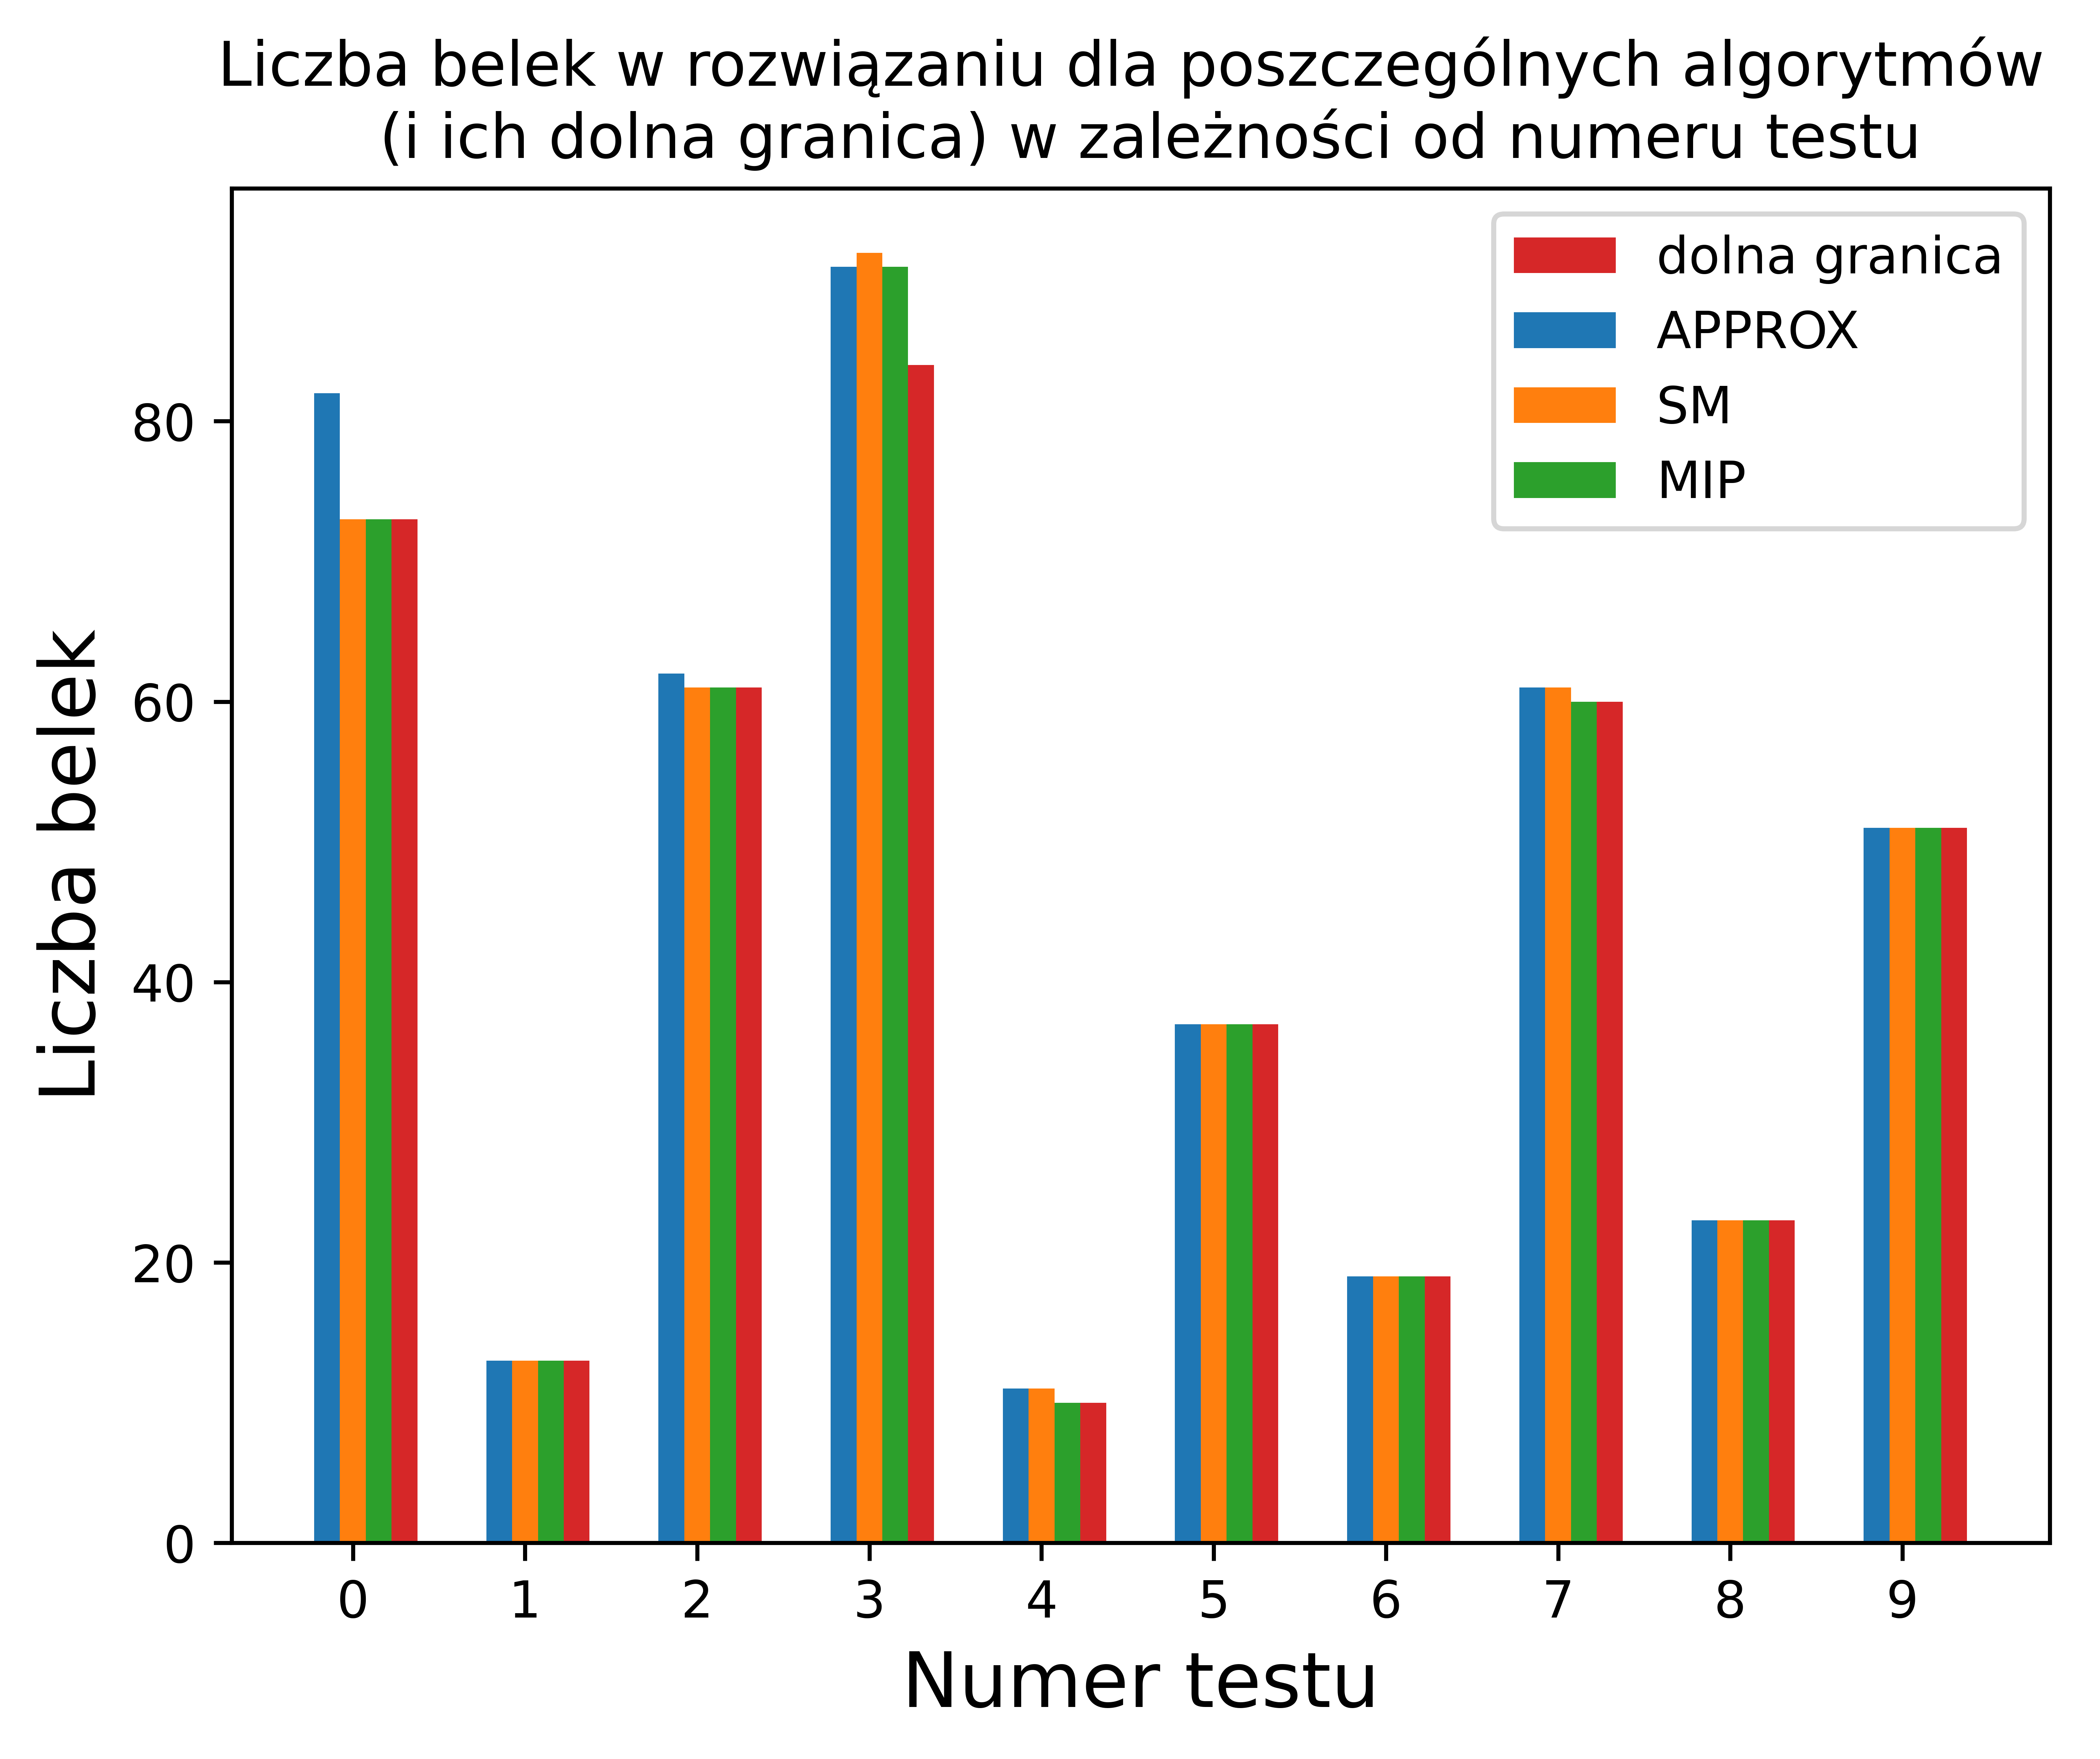
\includegraphics[width=12cm]{plots/res}
	\caption{Wykres przedstawiający liczbę belek (i ich dolną granicę) w rozwiązaniu dla poszczególnych algorytmów w zależności od numeru testu.}
	\end{center}
\end{figure}

\begin{figure}[H]
	\begin{center}
		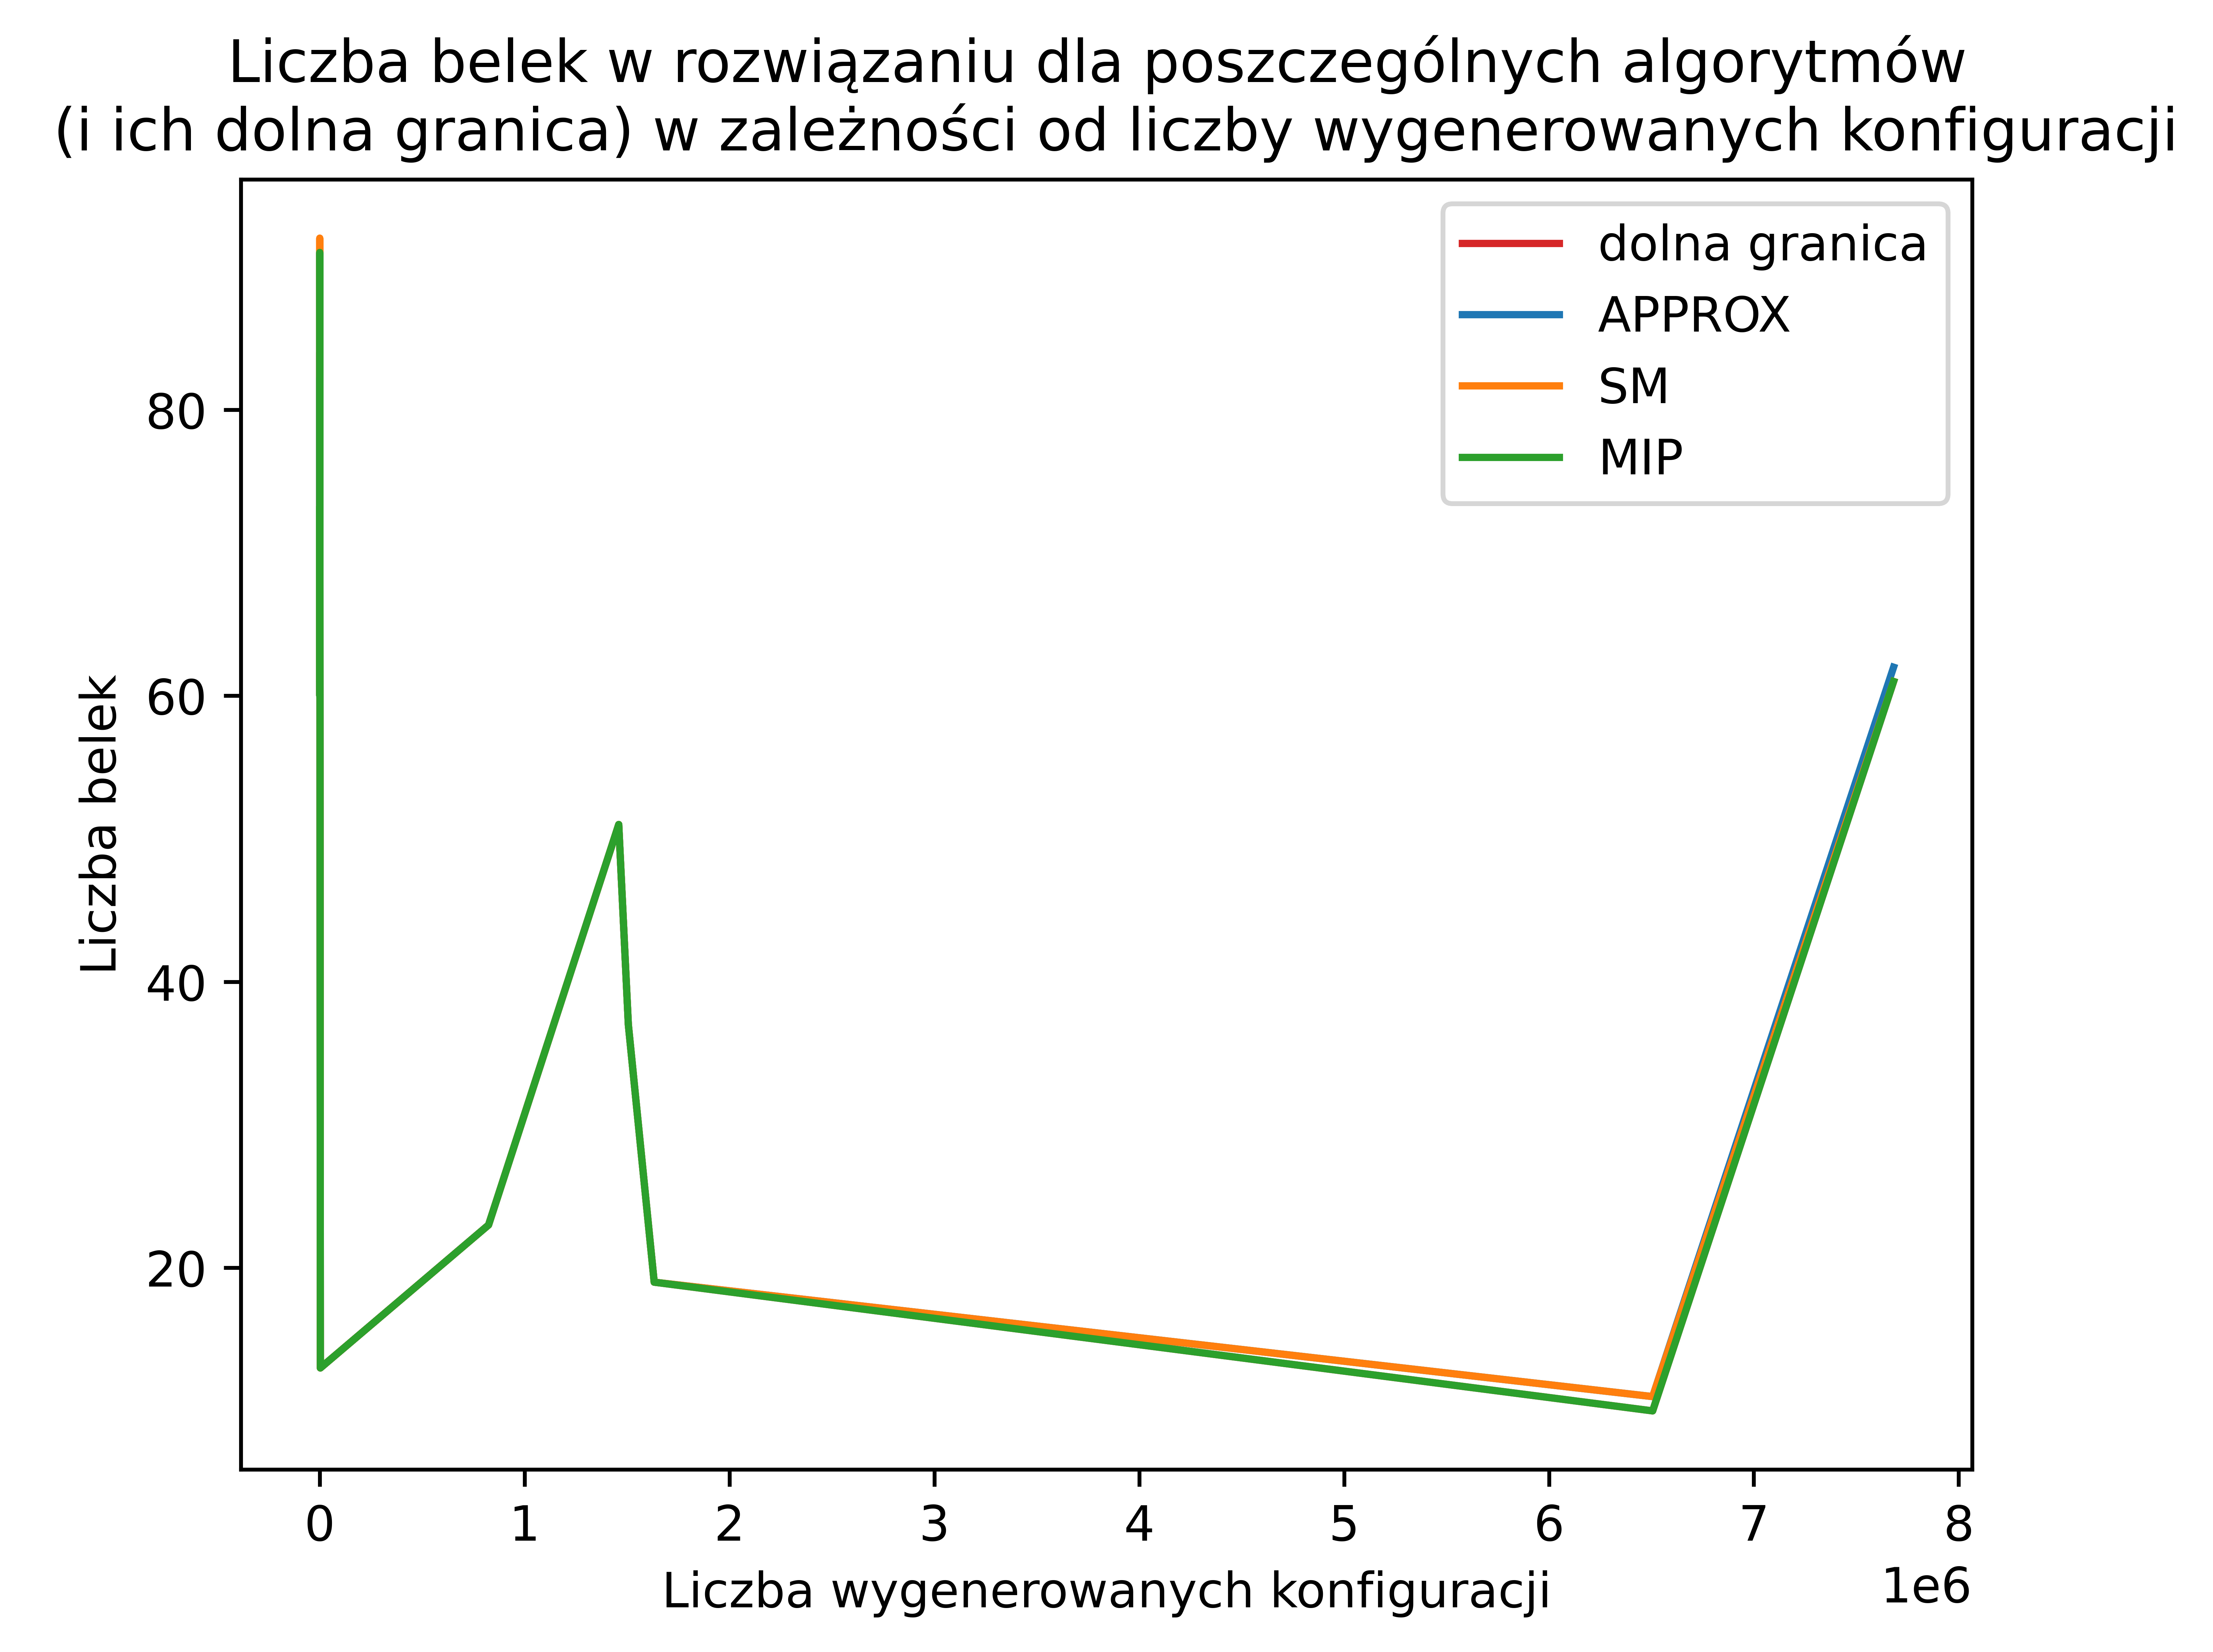
\includegraphics[width=12cm]{plots/res_configs}
		\caption{Wykres przedstawiający liczbę belek (i ich dolną granicę) w rozwiązaniu dla poszczególnych algorytmów w zależności od liczby wygenerowanych konfiguracji.}
	\end{center}
\end{figure}

\subsection{Czas wykonania}

\begin{table}[H] 
	\begin{center}
		\begin{tabular}{|p{3cm}|p{3cm}|p{3cm}|p{3cm}| } \hline
			Numer testu & APPROX & SM & MIP\\ \hline
			0 & 0.001 & 0.002 & 0.006\\ 
			1 & 0.001 & 0.004 & 0.055\\ 
			2 & 0.002 & 180.953 & 10076.226\\ 
			3 & 0.001 & 0.002 & 0.003\\ 
			4 & 0.001 & 7.963 & 1398.353\\ 
			5 & 0.002 & 4.625 & 1211.544\\ 
			6 & 0.001 & 4.218 & 779.089\\ 
			7 & 0.001 & 0.002 & 0.017\\ 
			8 & 0.001 & 1.720 & 434.735\\ 
			
			\hline
		\end{tabular}
		\caption{Czas wykonania progamu (w sekundach) dla poszczególnych algorytmów i testów}
	\end{center}
\end{table}

\begin{figure}[H]
	\begin{center}
		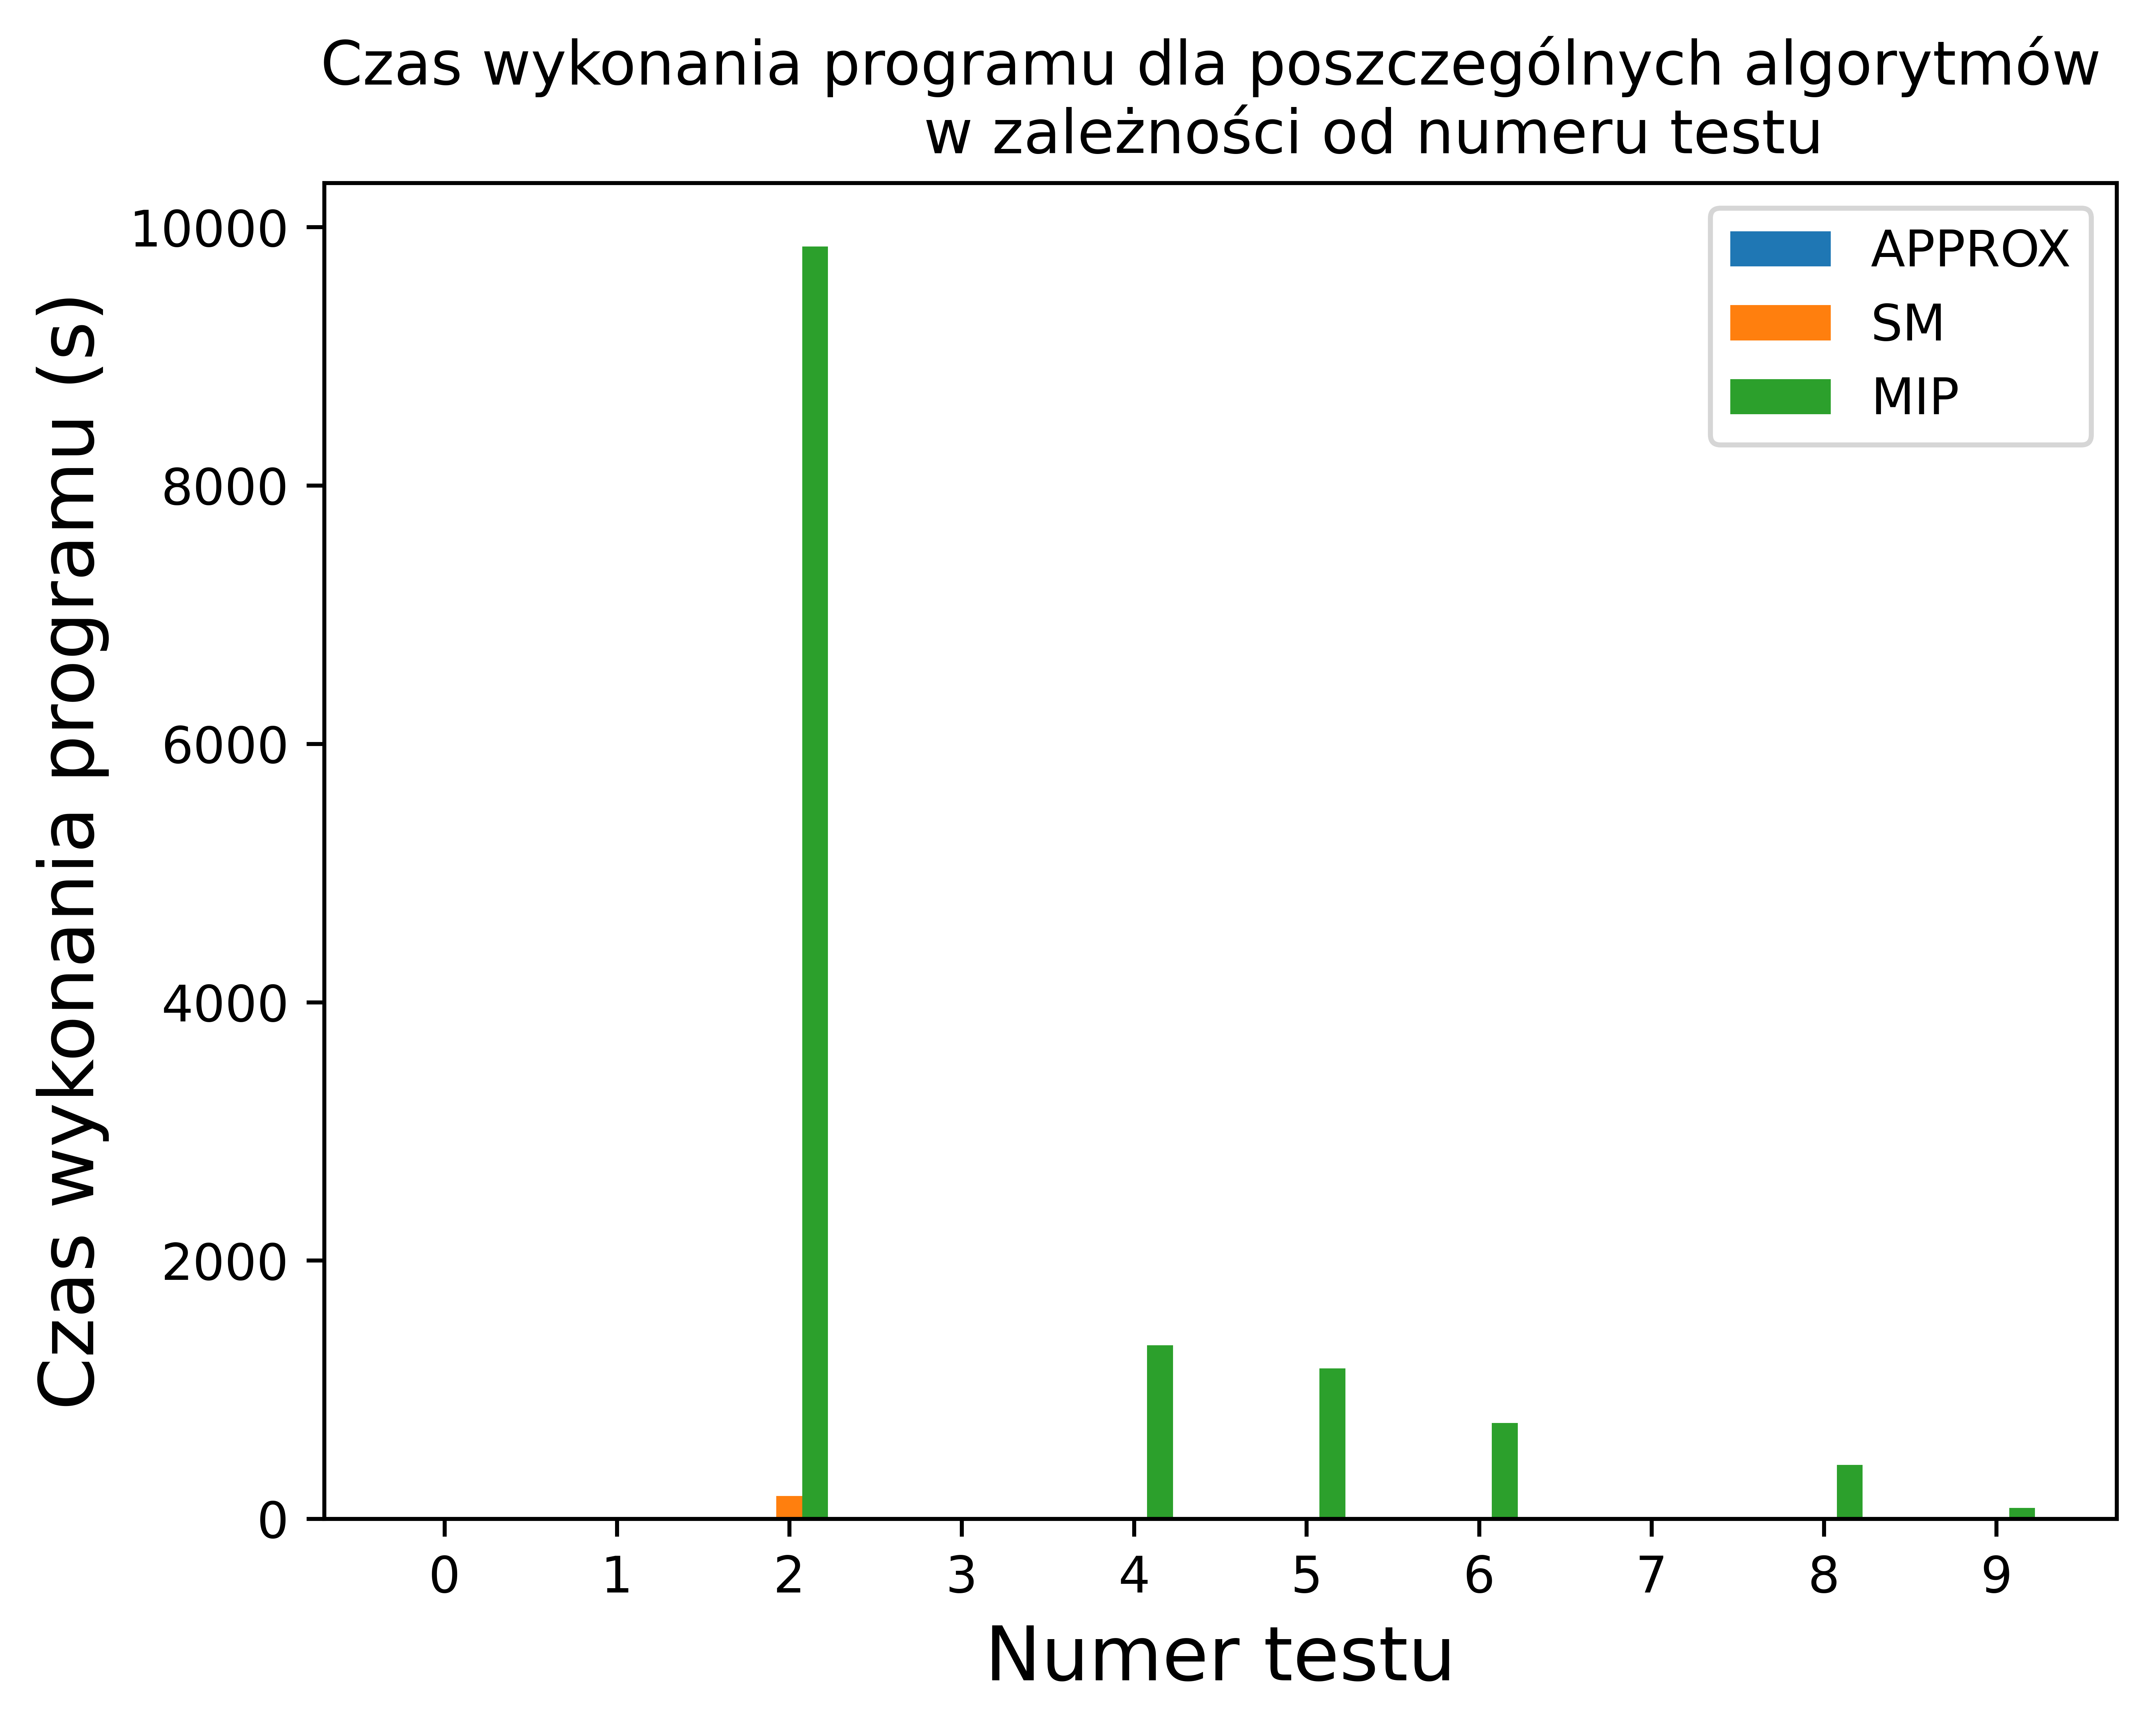
\includegraphics[width=12cm]{plots/time}
		\caption{Wykres przedstawiający czas wykonania programu dla poszczególnych algorytmów w zależności od numeru testu.}
	\end{center}
\end{figure}

\begin{figure}[H]
	\begin{center}
		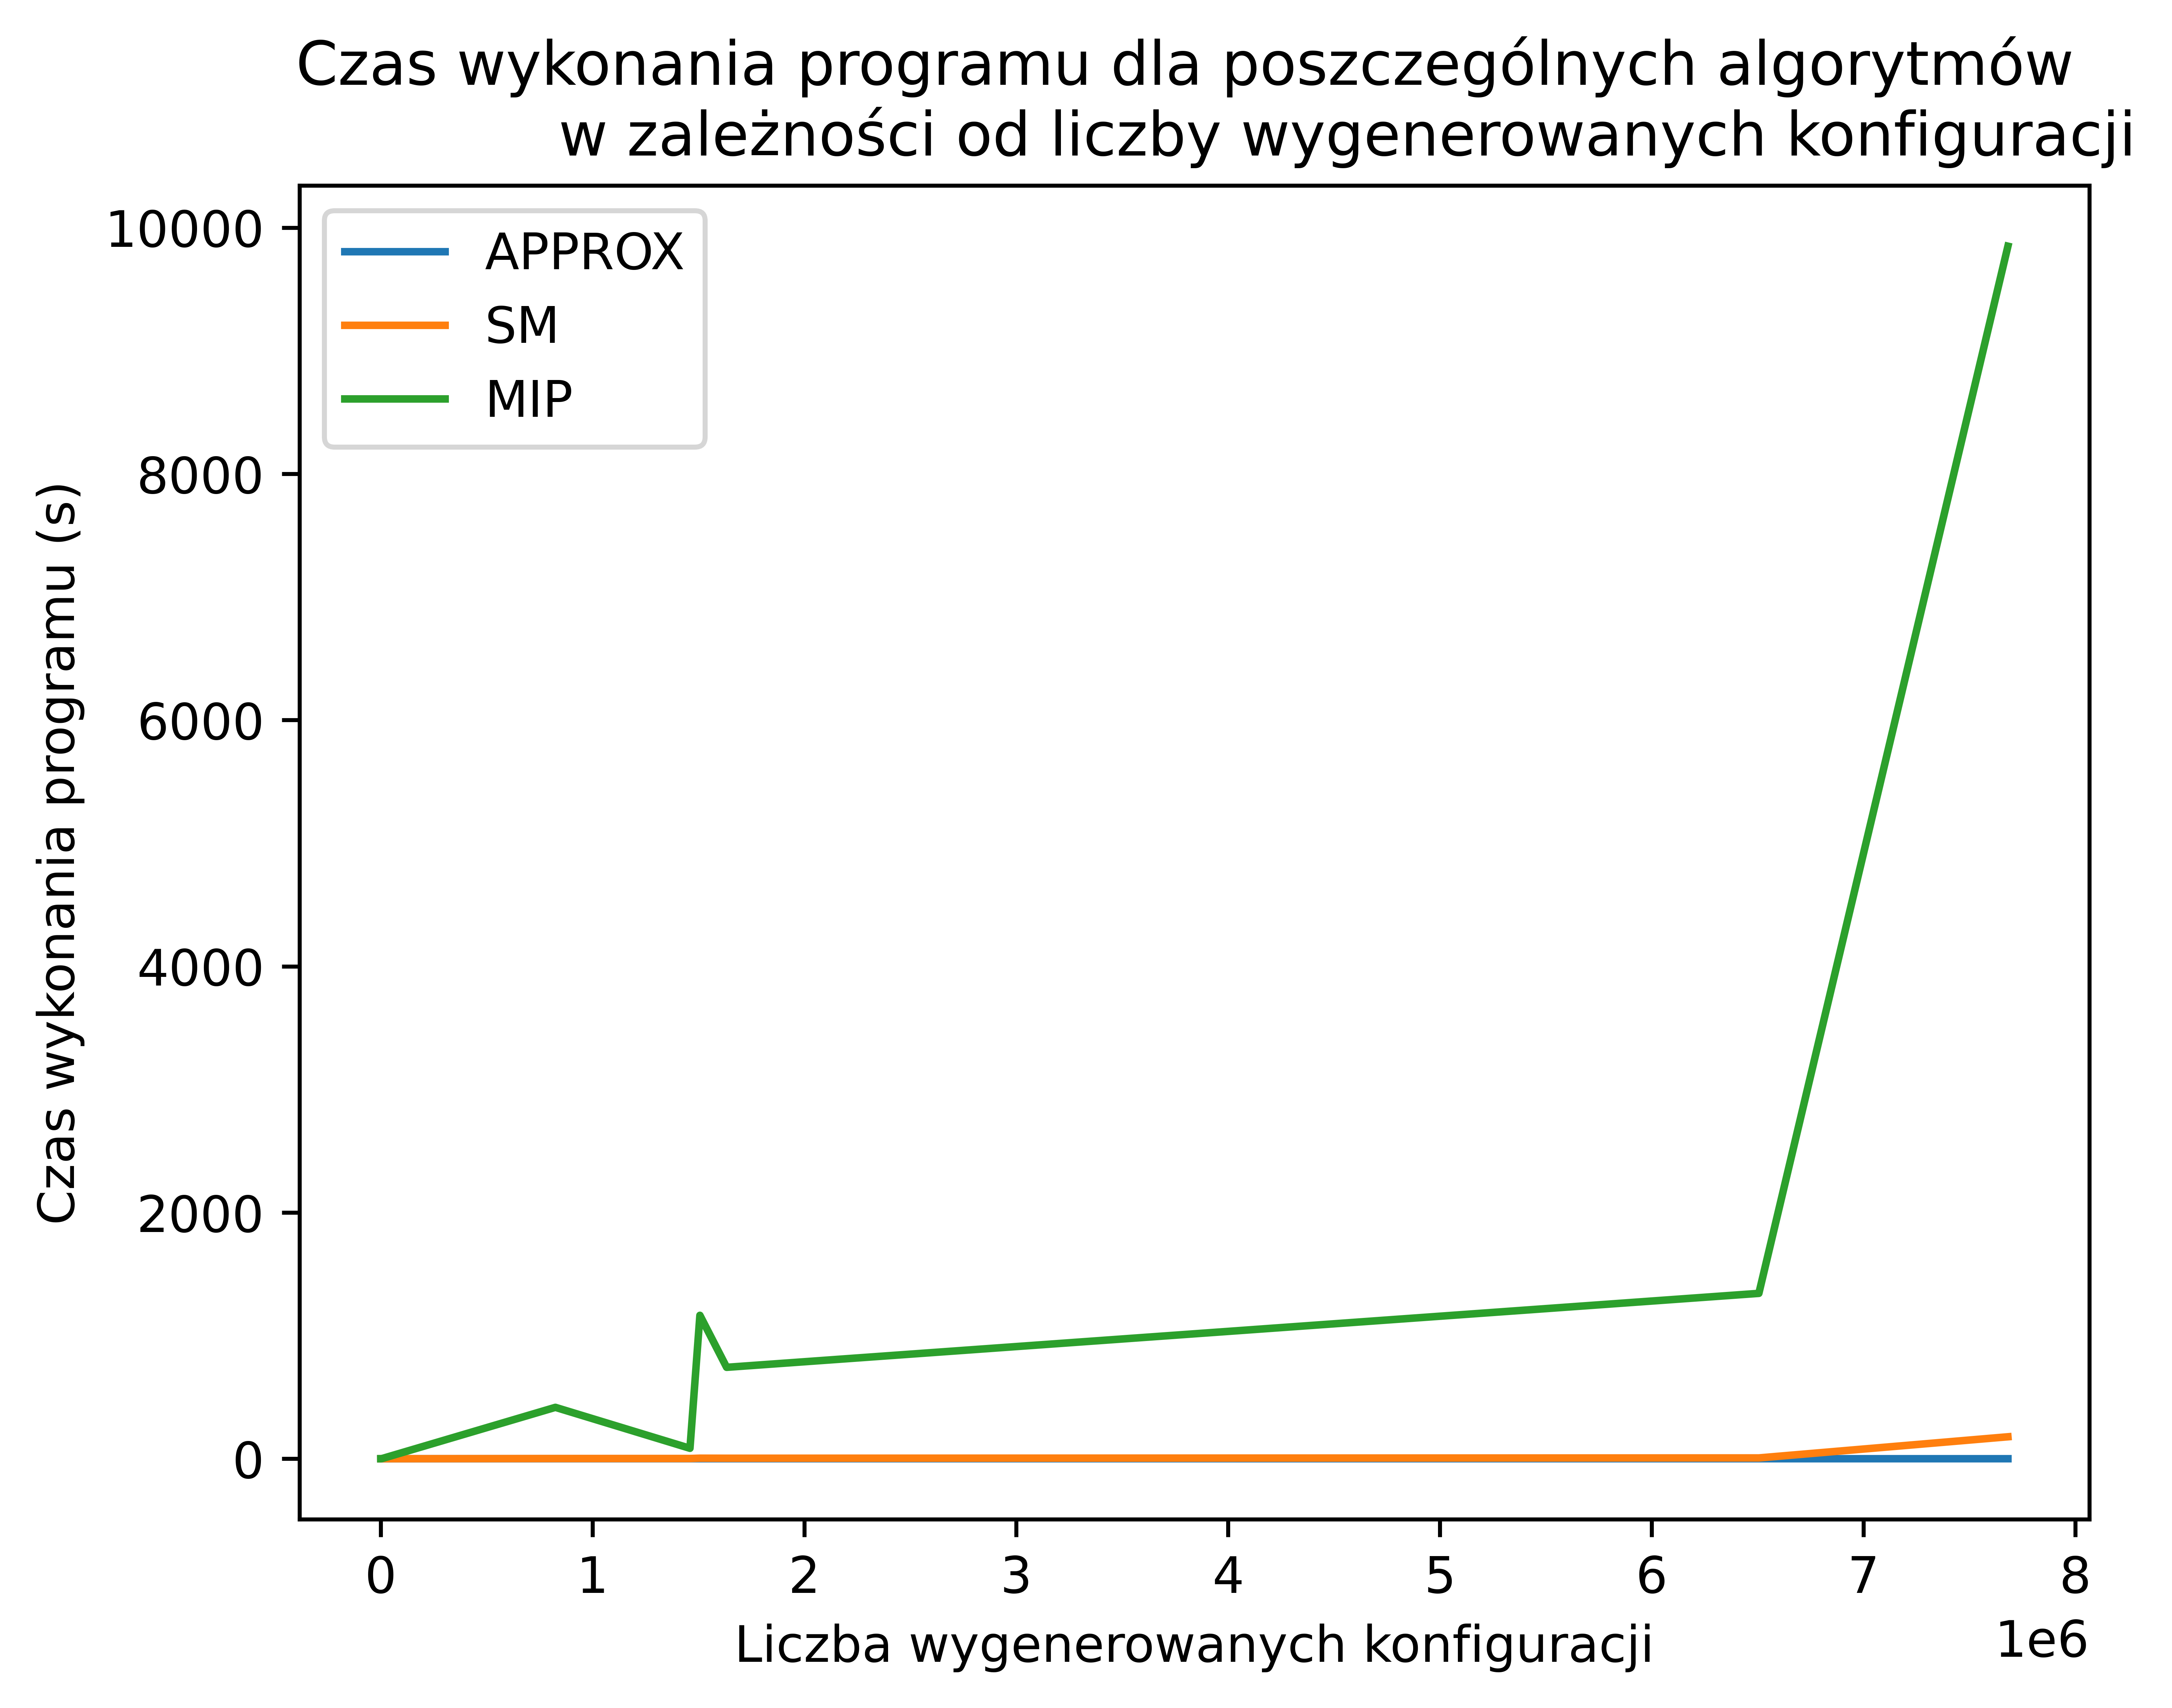
\includegraphics[width=12cm]{plots/time_configs}
		\caption{Wykres przedstawiający czas wykonania programu dla poszczególnych algorytmów w zależności od liczby wygenerowanych konfiguracji.}
	\end{center}
\end{figure}


\section{Wnioski}
Pierwszym co można zauważyć z zaprezentowanych powyżej danych jest to, że otrzymane rozwiązania są często blisko dolnej granicy. Jedynie w teście o numerze zero różnica ta wynosi aż dziewięc belek dla algorytmu aproksymacyjnego. Policzmy czy mieście się to we współczynniku aproksymacji: $73*11/9=89,(2) \leq 83$. Odpowiedź jest twierdząca. 
Drugią kwestią jest bardzo zróźnicowany czas działana algorytmów.
Program używający algolrytmu aproksymacyjnego nie przekroczył nigdy dwóch milisekund. Natomiast MIP potrafił działać nawet prawie 3h (test drugi - 10076.226s) zanim znalazł optymalne rozwiązanie. Jednak to nie sama optymalizacja liniowa powoduje taki narzut czasu. Gdy popatrzymy w teście piątym na algorytm SM, czas jego wykonywania jest prawie 261 razy krótszy ($1211.544÷4.625 \approx 261,95$). Nasuwa się tu wniosek, że to znalezienie rozwiązania optymalnego pod kątem całkowitoliczbowym jest za to odpowiedzialne (sekwencja branch-and-cut następująca po optymalizacji sympleksowej). 
Pierwszym wytłumaczeniem tego może być informacja zawarta w dokumentacji GLPK: \textit{GLPK branch-and-cut solver is not perfect, so it is unable to solve hard or very large scale MIP instances for a reasonable time.} 
Jednakże można zastanowić się czy algorytm approksymacyjny nie zwraca zadowalających wyników, skoro w powyższych testach tylko cztery razy był gorszy od MIP (w tym trzy razy różnica wynosiła jedną belkę). Gdyby jednak zależało nam na obsłużeniu skrajnych przypadków, SM radzi sobie w nich lepiej od samego aproksymacyjnego, podobnie do MIP, ale za to często w łatwych przykładach jest gorszy od tego pierwszego.



